\chapter{Data Center}

\section{Sie kennen die Building Blocks eines Datacenters}

Ein Datenblock besteht aus folgenden Building Blocks:

\begin{itemize}
	\item Server
	\item Speicher
	\item HVAC (heating, ventilation and air-conditioning)
	\item UPS (uniterruptible power supply)
	\item Redundanzen (verhindern eines “single point of failure”)
	\item angehobener Boden
	\item Feuerlöschsysteme (Argonit, FM-200)
	\item Physische Sicherheit (Zutrittsysteme, Aufsichtsperson)
\end{itemize}

\subsection{Fiber}
\begin{itemize}
	\item \textbf{Single-mode fiber}\\
		Werden für lange Strecken eingesetzt (bis 100km Länge) und hohe Übertragungsraten (bis 100Gbit/s). Die Glasfaser selbst ist nur 8-10.5 mikrometer dick. Der Lichtimpuls wird durch einen Laser erzeugt. Teurer.
	\item \textbf{Multimode fiber}\\
	Für kurze Strecken eingsetzt (On Campus, bis 500m Länge) und niedrigere Übertragungsraten (10Gbit/s). Der Lichtimpuls wird durch eine LED erzeugt. Günstiger.
\end{itemize}

\subsection{Downtime}
Downtime kostet, je nach Branche, extrem viel Geld. Das schlimmste wäre allerdings permanenter Datenverlust. Wenn nach einer Katastrophe wie 9/11 die Daten nicht innerhalb von 2 Wochen rekonstruiert sind, stirbt die Firma.
\begin{table}[h]
	\begin{tabular}{ll}
		\textbf{Uptime (\%)} & \textbf{Downtime}        \\
		90\%                 & 876 Stunden (36,5 Tage)  \\
		95\%                 & 438 Stunden (18,25 Tage) \\
		99\%                 & 87,6 Stunden (3,65 Tage) \\
		99,9\%               & 8,76 Stunden             \\
		99,99\%              & 52,56 Minuten            \\
		99,999\%             & 5,256 Minuten            \\
		99,9999\%            & 31,536 Sekunden         
	\end{tabular}
\end{table}
		99.9999\% sind von Firmen wie Google/Facebook/... erreicht.

\section{Sie wissen wie man Daten klassifiziert und sie in SLAs einbindet}

\subsection{Aktive vs. inaktive Daten}
Daten sind inaktiv, wenn sie nicht benutzt / gelesen werden und trotzdem gespeichert werden. Diese müssen genau wie aktive Daten gepflegt, archiviert, gesichert etc. werden.
Der Anteil an inaktiven Daten beträgt gegen 40\%. Da die Daten immer weiter wachsen, wächst auch der Anteil an inaktiven Daten mit. Teilweise kann man sich von den inaktiven Daten nicht entledigen. Beispielsweise kann es rechtliche Gründe haben wie das bei einer Krankenversicherung der Fall ist. Das Gesetz schreibt genau vor, wie lang welche Daten gespeichert werden müssen.
Der Anteil an inaktiven Daten kann mittels eines Life Cycle Managements verringert werden. Dabei könnte man definieren, dass Daten nach einer gewissen Zeit ohne Zugriff automatisch gelöscht werden. Aber Achtung: Dies passt nicht zur Philosophie von Big Data (möglichst alles speichern und für immer).

\subsection{Datenklassen}\label{sec:datenklassen}

\begin{itemize}
	\item \textbf{Mission Critical Data} \\
	Muss schnell sein, hochverfügbar, redundant usw.
	\item \textbf{Business Critical Data} \\
	Geschäftskritische Daten einer Applikation (Geschäftsapplikation)
	\item \textbf{Nearline Data} \\
	z.B. E-Mail
	\item \textbf{Offline Data} \\
	Daten auf welche nicht direkten Zugriff erwartet wird. z.B. E-Mail Archivierung für Compliance. (u.a. Tape)
\end{itemize}

\begin{figure}[h!]
	\centering
	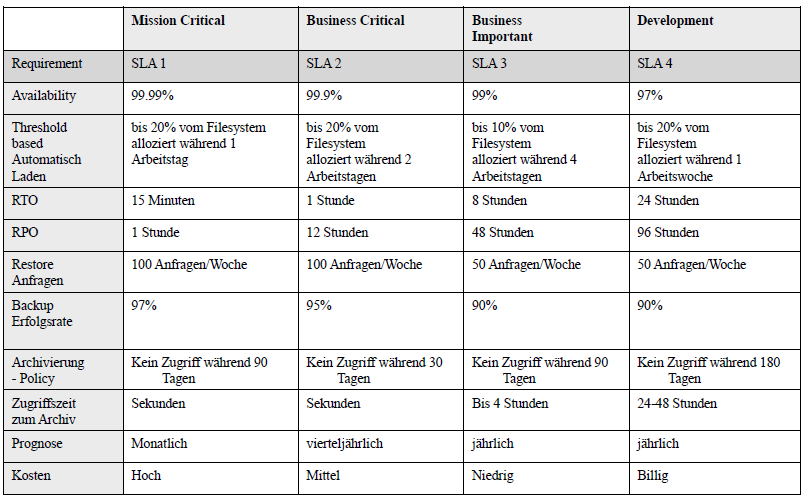
\includegraphics[width=0.9\linewidth]{fig/sla}
	\caption{Beispiele für SLAs}
	\label{fig:sla_beispiele}
\end{figure}

\section{Sie sind in der Lage Data-Tiers und deren Aufgaben zu erklären}

\subsection{Data Tiers}\label{sec:storagetier}

\begin{itemize}
	\item \textbf{Tier 1}
		\subitem Höchster Speed, sehr zuverlässig, hohe Skalierbarkeit, sehr teuer. Wird von Mission Critical Data benutzt.
		\subitem 20\% aller Daten 
		\subitem SSDs oder FC/SAS Platten
	\item \textbf{Tier 2}
		\subitem Mittlerer Speed, okay zuverlässig, limitiert skalierbar, nicht so teuer. Wird von Business Critical Data verwendet.
		\subitem FC/SAS Platten
	\item \textbf{Tier n}
		\subitem Hohe Kapazität, allerdings niedriger Speed, sehr günstig. Könnte als Nearline-Storage verwendet werden (d.h. E-Mail)
		\subitem 35\% aller Daten
		\subitem Commodity Festplaten (SATA)
	\item \textbf{spezialisiert}
		\subitem Offsite / Offline Tape Archivierung (15\% aller Daten)
		\subitem Einmal Beschreibbare Medien (für Compliance) (30\% aller Daten)
		\subitem Tape oder MAID
\end{itemize}
Tape Archivierung ist immer noch das billigste Archiv-Medium und der vielseitigste Archivierungs-Speicher den es gibt. Allerdings ist Archivierung kein Backup!

\begin{figure}[h!]
	\centering
	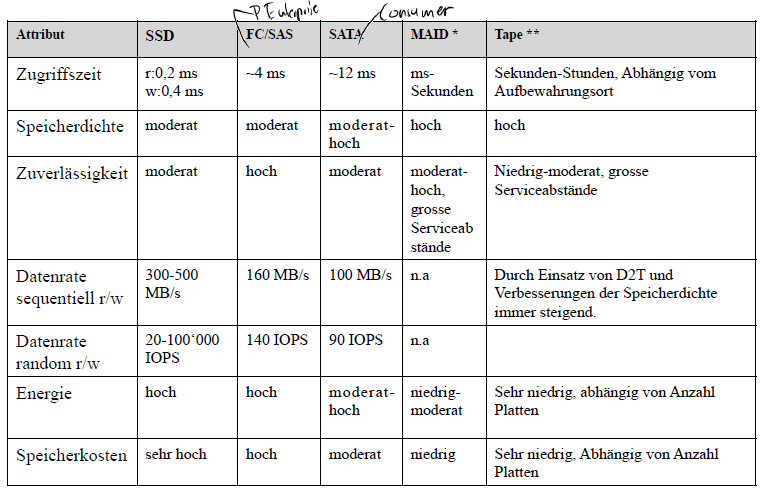
\includegraphics[width=0.9\linewidth]{fig/speichertypen}
	\caption{Übersicht Speichertypen}
	\label{fig:speichertypen}
\end{figure}

\subsection{MAID}\label{sec:maid}
Meint \emph{Massive Array of Idle Disks}. Wird eingesetzt bei Archivierungslösungen, bei denen auf Festplatten archiviert wird. Daher wird nicht häufig auf diese zugegriffen, was bedeutet, dass diese auch abgeschaltet werden können und bei Bedarf wieder hochgefahren werden können. Das bedeutet Stromersparnis - wichtig bei Green IT.

Beim Lesen muss gewartet werden, bis die korrekte Festplatte hochgefahren wurde. Das Schreiben geschieht auf einen Cache, oder auf eine zufällig laufende Festplatte. Danach wird die korrekte Festplatte hochgefahren und die Daten dorthin verschoben.

\subsection{Information Lifecycle Management (ILM)}
Verschiebung der Daten von Tier 1 bis Tier n (oder zur Löschung), mit dem Ziel der Optimierung der Kosten in der IT. Verschiebung anhand Kriterien wie Kosten, Ökonomischer Wert, Speicherzeit, letzter Zugriff, Anforderung an Zugriffsgeschwindigkeit oder auch gesetzliche Bestimmungen.

\subsection{Speicherallokation / Effizienz}\label{sec:speichereffizienz}
\begin{itemize}
	\item \textbf{allocation} \\
		Speicherplatz der vom System reserviert wird. Problematik, da man nicht vorhersagen kann, wie viel Speicherplatz von der Applikation effektiv verbraucht wird. Kann durch thin provisioning in den Griff bekommen werden.
	\item \textbf{utilization efficiency} \\
		Effektiver Ausnützungsgrad des reservierten Speichers. Hier ist es auch wichtig, dass die Daten auf dem passenden Tier gespeichert - Emails haben nichts auf Tier 1 verloren. 
	\item \textbf{storage yield} \\
		Bedeutet so viel wie \emph{Speicherausbeute}. Beschreibt, wie viel vom alloziiertem Speicher effektiv belegt ist.
	\item \textbf{COPQ} \\
		Bedeutet \emph{Cost of poor quality}. Beschreibt die Differenz zwischen den gesamten Kosten für ein Speichersystem (Unterhalt + Anschaffung) und den Kosten, welche durch den effektiv belegten Speicherplatz relativ dazu entstehen. Beispiel; 2TB Platte kostet bei digitec.ch 100CHF, davon braucht man aber nur 300GB, dann wären die COPQ 70CHF.
\end{itemize}

\section{Sie sind fähig die kritischen Punkte eines Datacenters zu adressieren und Massnahmen vorzuschlagen}
Wenn man die Qualität verbessern will, muss man auch die Verfügbarkeit erhöhen. Diese erhöht man nur durch Redundanz.

\subsection{Replikationsarten}\label{sec:replikationsarten}
\begin{itemize}
	\item \textbf{Synchron} \\
		Speichersystem / Datenbank liefert OK erst zurück wenn die Daten auf beiden Systemen persistiert wurden. Dies funktioniert nur, wenn beide Systeme relativ nahe beieinander liegen.
	\item \textbf{Asynchron} \\
		System liefert OK schon zurück, wenn Daten auf einem einzigen System geschrieben wurden und repliziert die Daten im Hintergrund auf das entfernte System. Funktioniert über weite Distanzen tiptop.
	\item \textbf{Kombination Asynchron / Synchron} \\
		Die primäre Datenbank schreibt alle Daten synchron auf eine kleine, lokale Zwischenstation. Diese Zwischenstation übernimmt anschliessend asynchron die Übertragung auf den entfernten Speicher.
\end{itemize}

\subsection{Beispiele für Redundanz}\label{sec:bsp_redundanz}
\begin{itemize}
	\item SANs Redundant halten (inkl. der Pfade zu den SANs).
	\item Failover Datacenter \\ 
		Das gesamte Datacenter ist gespiegelt vorhanden. Schwierig zu realisieren, da alles doppelt vorhanden sein muss - entsprechend teuer.
\end{itemize}
Ein Echtzeit-Switch zwischen Aktiv- und Failoverdatacenter ist nie möglich, da durch die Übertragungszeit immer eine Latenz im Spiel ist und daher die entfernte Datenbank im Grunde genommen immer inkonsistent ist.